\section{Verification, qualification and performance methodology}
\subsection{Different questions require different evidence}
The release checks the following separately:
\begin{enumerate}
\item Local kernels: collision/rate units, positive reaction maps, charge
 ledger, Bernoulli/vacuum limits and exponential drag weights.
\item Geometry/reconstruction: traced magnetic geometry, mapped-volume
 moments, cubic reproduction and bounded face reconstruction.
\item Elliptic algebra: manufactured tensor potential, regional/periodic
 boundaries and the explicitly recomputed true residual.
\item Transport/AMR: constant tracer, shared contacts, conservative
 density/momentum remap and the three physical-level entry paths.
\item Ownership: simultaneous/cross-peer molecular migration, round trips,
 exact no-op behavior and preservation of old owned state through remap.
\item Integration: fresh four-worker three-level and night-chemistry
 workflows, plus AddressSanitizer/UndefinedBehaviorSanitizer checks.
\item A developed-state qualification: complete saved-field and actual
 density-mask parity over the same physical interval, with full-process
 wall timing and separate resource accounting.
\end{enumerate}
Passing one does not replace the others. A 0.2 s teaching workflow validates
entry, coupling and output, not nonlinear bubble growth. Morphology is not
established by a rank count, residual or matching diagnostic scalar.

\subsection{The developed-state paired case}
The qualification continues one verified native/molecular checkpoint at
13350 s to 13500 s. User physical roots are 64 by80 with 64 field segments;
the three-level canonical geometry is256 by320 by64. The field is IGRF-14
at 2025.0, apex-longitude centre112.25 degrees and span8 degrees, spherical
apex range250--1600 km and conjugate base90 km. The frozen case retains
PDM4 with $\beta=1$, CFL 0.25, dt maximum 2 s, potential request $10^{-10}$,
the same transported-night closure, neutral inputs, seed/driver history,
structure thresholds, buffer 1, slab 4 and quiet 60 s. Output/checkpoints are
every 150 s, including initial and final frames.

The reference is the previously qualified owned-migration/log-cache version,
not the older production implementation. Old/new metadata-only source
bindings are audited in isolated copies; all physical payload bytes remain
unchanged. Geometry/IGRF token parity justifies annotation-induced identity
rebinding, with original hashes retained. Runtime readers still enforce
their exact identities. This is a validation conversion, not a public
restart bypass.

Within each allocation, one reference 64-by-1 launch precedes optimized 64-by-1,
32-by-2 and64-by-4 launches. The same 256 CPUs are reserved on two nodes, but
the active thread totals are 64,64,64 and256. Affinity probes precede model
launches and are excluded from model timing. The immediate synchronous
wait includes process start, geometry/cache/state initialization, output,
checkpointing and actual MPI exit. No PMPI observer is preloaded in any
of these launches. This differs from the earlier separate PMPI-observed
qualification; its absolute times must not be mixed into a new ratio.

Each field/component is compared with
\begin{equation}
 \epsilon_\infty=\frac{\max|q-q_{\rm ref}|}{\max|q_{\rm ref}|},
\end{equation}
scaling momentum components independently. This is a global-amplitude
normalization, not pointwise relative error near zero. Complete densities,
momenta, potential and reconstructed display fields at both saved times
are checked, and physical AMR level maps must be byte-identical. Conservation
and true residual must independently satisfy their acceptance criteria.

\subsection{Measured release qualification}
\noindent\textbf{Frozen numerical source ID.} \nolinkurl{b876245d6051ff517b9121fd6644ecafd762d5ff55ef5c3965895b8edd264c5d}\par
The frozen candidate completed all listed gates with zero compiler warnings.
Table~\ref{tab:perf} reports the complete matched launches on one two-node,
256-reserved-CPU allocation.

\begin{table}[ht]
\centering\small
\begin{tabular}{lrrrrr}
\toprule Variant & MPI & Workers & Active & Full wait(s) & Ratio \\ \midrule
reference64 & 64 & 1 & 64 & 499.981 & 1.000 \\
optimized64 & 64 & 1 & 64 & 481.027 & 1.039 \\
hybrid32x2 & 32 & 2 & 64 & 537.712 & 0.930 \\
hybrid64x4 & 64 & 4 & 256 & 374.899 & 1.334 \\
\bottomrule
\end{tabular}
\caption{Complete 13350--13500 s launches, including initialization,
outputs/checkpoints and actual process exit. Ratio is reference time divided
by row time. Every row reserves 256 CPUs, but active thread totals differ.
One launch per row; no statistical uncertainty estimate.}\label{tab:perf}
\end{table}

The same-active-thread64-by-1 implementation edit reduces full wait by
3.8\%. The fastest measured variant is
\code{hybrid64x4}, with 256 active threads; its
1.334 ratio is not a same-active-core algorithmic speedup.
The 32-by-2 configuration is slower than64-by-1 on this grid.
All saved-field checks pass; the largest global-amplitude-normalized
error is $6.765\times10^{-13}$, and actual AMR maps are byte-identical at both
frames. Completed true-residual and O$^+$ conservation checks also pass.
The new rank0 counters expose 400 accepted steps, 799 attempts, 399
initial CFL adjustments, 1200 RHS calls, 1199 chemistry calls and 41 tag
checks, with zero reported predictor/corrector failure retries. These
counts begin after the initial snapshot and include terminal diagnostic
RHS work. The release retains the stability/retry policy.

The exact source/build/input hashes, effective parameters, per-field errors
and completed diagnostics are recorded in \path{validation/qualification.json}.
Earlier separately paired candidate measurements are retained as history,
not mixed into the current speed ratio.


\begin{figure}[ht]
\centering
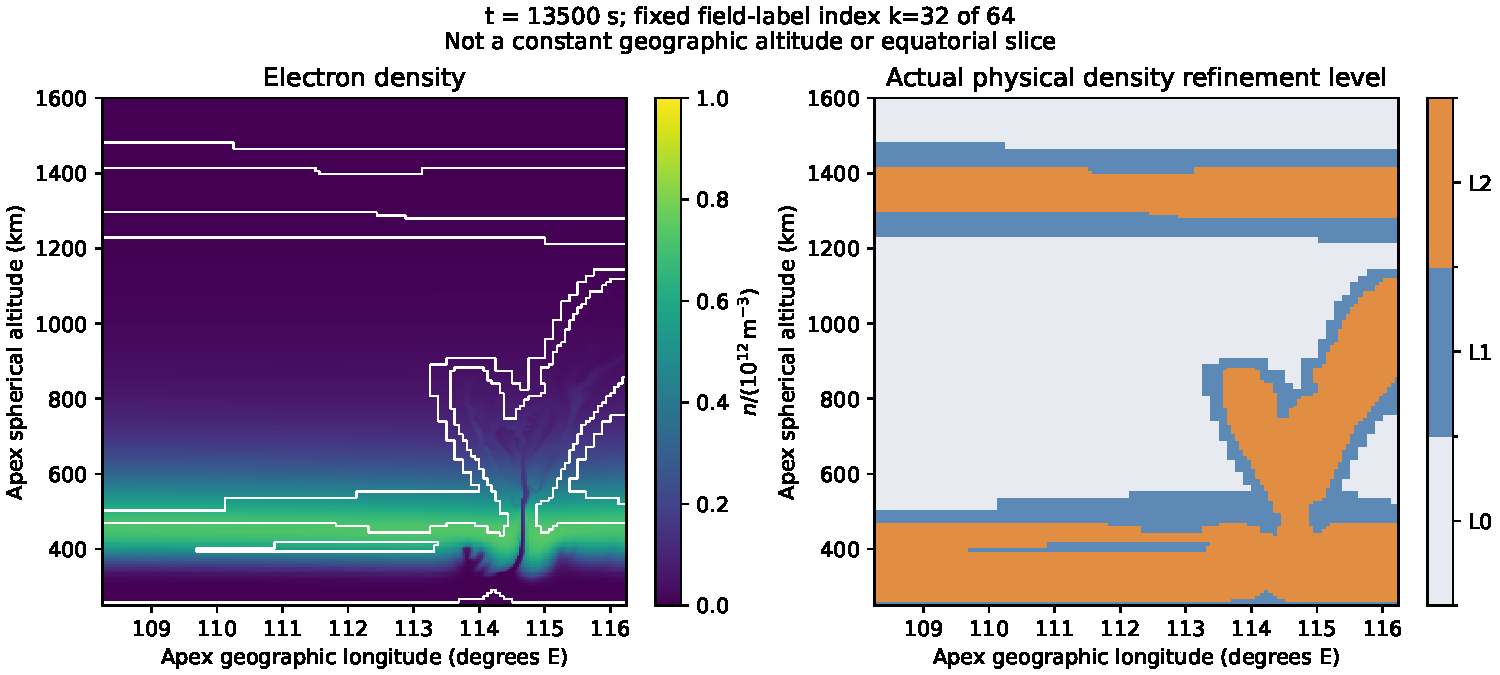
\includegraphics[width=\linewidth]{images/qualified_slice.pdf}
\caption{Saved 13500 s electron density and actual physical density-refinement
levels from the qualified 64-by-1 candidate. This is a fixed field-label-index
slice ($k=32$ of 64) plotted against apex longitude and spherical apex altitude;
it is neither an equatorial plane nor a constant geographic altitude cut.
Ne includes both molecular species. White digital cell-edge outlines separate
actual physical refinement levels; individual fine-grid cells are omitted.
Canonical O$^+$ detail in coarse regions is conservative display reconstruction,
not an independently evolved fine degree of freedom. Colors are clipped at
$10^{12}\,\mathrm{m^{-3}}$ for display only. Input/plot hashes and library versions
are recorded with the figure. No model integration was repeated to create it.}
\label{fig:saved-state}
\end{figure}

\subsection{Timing scope and retained failures}
Completion phase counters are rank-local and overlap: regrid includes
prepare/solve, and the legacy chemistry timer includes response refresh
and molecular halo wait. Terminal diagnostic RHS can be included in those
counters while the evolution interval timer ends before the last snapshot.
They are not an exclusive additive timeline. Independent phase maxima
must not be subtracted to claim an optimization. GNU-time CPU usage can
include MPI busy waiting and does not prove useful load balance.

Single paired launches have no repeated-run uncertainty estimate and are
not extrapolated to 20000 s production wall time. Increasing active workers
is distinguished from same-active-thread code/decomposition gains. All
successful states, failed gates/submissions and logs are preserved. A
reader/plot repair uses saved outputs rather than replaying a successful
scientific process. Production jobs and their controller are independent
of these isolated short qualifications and are not interrupted or modified.

\subsection{Evidence still needed for scientific publication}
This methods release does not claim a measured convergence order or exact
TELF validation, and none is inferred from PDM4's cubic stencil. Suitable
science studies should establish resolution sensitivity of the actual
depletion/branch observables, background/driver sensitivity, domain and
boundary influence, and observation sampling on actual ECEF geometry.
Hong Kong/Sanya ISR comparisons require electron rather than O$^+$ density,
appropriate height/beam coverage, correct local-time interpretation and
event-specific background provenance. Those studies are distinct from
demonstrating that a performance edit preserves an existing computation.
